\chapter{Probabilistic Score}
\label{chap4}
This paper proposes a departure from the previous cost function definitions, looking instead at using a probabilistic model to directly estimate the likelihood of two edges matching.
\section{Motivation}
A pervasive problem with the cost functions discussed above is that their design is ad hoc and relies on hand-picked values based on the authors' empirical observations. For instance, in \cite{P1} the authors have to decide on the size of the Gaussian window they employ, on the weights to assign to the pixels that fall within that window and on a suitable value for their threshold function. \todo{Explain these cost methods in the lit. review} In \cite{P2} the authors not only face all of the above problems, but also have to decide on a threshold value for their row comparison and on another threshold regarding the minimum amount of black pixels that an edge must have in order for it's matches to be considered relevant. 

This ad-hoc formulation suffer from several impediments which the probabilistic method manages to avoid or at least ameliorate:
\begin{table}[h]
  \centering
  \begin{tabular}{p{0.5\textwidth} | p{0.5\textwidth}}
  Cost function & Probabilistic score function \\ \hline
Relies on the values the authors hand-picked for their particular dataset & Learns a new document's pixel distribution by analysing the shreds it is given \\ \hline
Cannot be easily combined with a different similarity function, as it lacks modularity & Can be easily composed with any similarity function that produces a probability. Several such functions already exist, such as the optical character recognition based system proposed in \cite{P8}) \\ \hline
  \end{tabular}
  \label{tab:costScoreComp}
\end{table}
\begin{table}[h]
  \centering
  \begin{tabular}{p{0.5\textwidth} | p{0.5\textwidth}}
  Cost function & Probabilistic score function \\ \hline
Difficult to evaluate results of the function since the numbers outputted are meaningless, only the order of the results matters & The scores returned are the estimated probabilities of matching, so evaluation is natural, by comparing estimated and observed probabilities. \\ \hline
Cost is additive and must therefore be normalized relative to the sum of lengths of the matching edges & All scores are normalized probabilities, so length of edges or number of edges matching is irrelevant (see Figure x)  \\ \hline
  \end{tabular}
  \label{tab:costScoreComp}
\end{table}
\missingfigure{Add figure explaining cost normalization for multiple edges}

Lastly, the effectiveness of probabilistic models, when applied to text data, has been repeatedly shown. Pixel prediction goes back to systems such as the 1981 JBIG lossless compression ISO standard( which tried to predict the value of a pixel using several features including 6 of it's neighbours \cite{P3} ) and is still employed in today's state of the art encoders \cite{P4}. 

\section{Description}

The central idea of the probabilistic function is, when looking at a proposed match, to estimate the probability that a candidate pixel is correct given several of its neighbour pixels(i.e. the candidate pixel's "context", see Figure \ref{fig:probContext}). We refer to this conditional probability as \(\Pr( p \mid C(p,E_x) )\), where \(C(p,E_x)\) is the context of pixel $p$ when placed next to edge $E_x$. Ideally we'd want to learn these conditional probabilities by analysing the original document, which we obviously don't have access to. However, relatively few pixels are destroyed when shedding a document and we can assume that the ones that are destroyed are uniformly distributed over the space of contexts. Therefore the cumulative distribution of the shreds will, in general, be a close approximation to the distribution in the original document, which means we can get a good estimate of the needed probabilities by analysing each individual shred and averaging the results.

\begin{figure}[h]
\centering
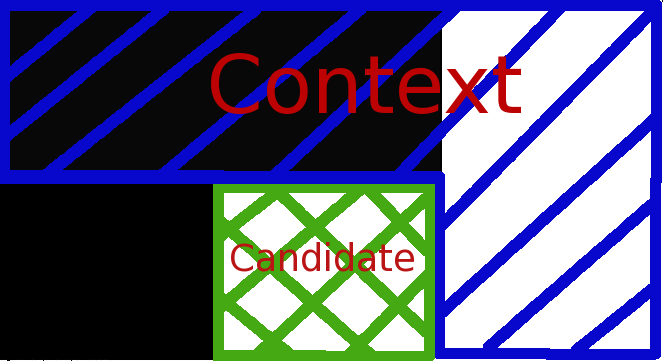
\includegraphics[width=0.8\textwidth,height=5cm]{context}
\caption{This shows a proposed match between the top 3 and the bottom 3 pixels. The model estimates the probability that the candidate pixel is white based on the four context pixels}
\label{fig:probContext}
\end{figure}

\subsection{Edge likelihood}

Once we have estimated the conditional probabilities, the total probability of two edges matching can be calculated by sliding the context down the proposed edge and multiplying all the individual candidate pixel probabilities. That is to say, if we have a proposed matching between edge \(E_1\) and edge \(E_2\), and \(E_1^x\) represents the $xth$ pixel on edge 1, then we would estimate: \[\Pr(E_1,E_2) = \prod_{i=1}^{len(E_2)} \Pr(E_2^i \mid C(E_2^i,E_1))\] A problem arises though, because the shape of the context prohibits us from taking the conditional probability for the first and last few pixels (depending on the length of the context). For these the best we can do is assign them the prior probability, \(\Pr(p)\), which is also extracted from the data simply by counting the proportion of white and black pixels. Therefore, when using the context of size 4 shown in Figure \ref{fig:probContext}, the edge probability will actually be\footnote{There actually is a further problem with the presented formula, namely that it doesn't account for edges belonging to the same piece. If \(E_1\) and \(E_2\) both belong to the same shred then obviously the probability that they match is 0 since a shred can't be in 2 places at once. This extra complication is ignored in the mathematical formalism for reasons of clarity}  \[\Pr(E_1,E_2) = \Pr(E_2^1) \Pr(E_2^{len(E_2)}) \prod_{i=2}^{len(E_2)-1} \Pr(E_2^i \mid C(E_2^i,E_1)) \]

\subsection{Normalization}\label{sect:norm}
The above, while being a good measure of the likelihood of an edge, is a function that will tend to decrease as $len(E_2)$ increases. The function will therefore tend to prefer shorter edges with less probabilities to multiply. Luckily, using probabilities gives us one more piece of information here. In the original file, every edge of every shred has only one correct match, since no two shreds are superimposed. Therefore, we know that the sum of the probabilities of all matches along one edge should sum up to one. In technical terms, if \(S_E\) is the set of all edges, then: \[\forall E_a \sum_{E_x \in S_E} \Pr(E_a,E_x) = 1 \] In order to satisfy this constraint the probabilities are normalized along every edge. After the normalization, the preference for shorter edges is eliminated and the probabilities for different edges and pieces can be directly compared regardless of local features such as a particular edge length. Therefore, accounting for the normalization process, the final definition becomes:  \[ \Pr(E_1,E_2) = \frac{\Pr(E_2^1) \Pr(E_2^{len(E_2)}) \prod_{i=2}^{len(E_2)-1} \Pr(E_2^i \mid C(E_2^i,E_1))}{\sum_{E_x \in S_E} \Pr(E_x^1) \Pr(E_x^{len(E_x)}) \prod_{i=2}^{len(E_x)-1} \Pr(E_x^i \mid C(E_x^i,E_1)) } \]


The normalization discussed above has an additional property, which ends up mitigating the predisposition towards whitespace that some of the other cost functions suffer from. \todo{explain this predisposition in lit. review} The property in question is that if \(E_1\), \(E_2\) and \(E_3\) are very similar or identical edges then they will have less chance of being picked as the best match because the available probability mass of any match will be split equally among the 3 of them. Formally, if \(I_{E_x}\) is the set of edges identical to \(E_x\) then: \[\forall E_a \Pr(E_a,E_x) \leq \frac{1}{\mid I_{E_x} \mid}\] Since there are usually several white edges floating around in the edge set at any time, the above property ends up naturally discounting them without the need for any ad hoc heuristics (see Table \ref{tab:normalization} for a typical situation). To further discount the white on white matches we can introduce dummy white pieces into the shreds pool.

\begin{table}[h]
  \centering
  \begin{tabular}{|c|c|c|c|c|c|c|}
    \hline
    & \multicolumn{3}{|c|}{Raw probabilities} &  \multicolumn{3}{|c|}{Normalized probabilities} \\
    \cline{2-7}
    & Edge 3 & Edge 4 & Edge 5 & Edge 3 & Edge 4 & Edge 5 \\
    \hline
    Edge 1 & 0.90 & 0.90 & 0.20 & 0.45 & 0.45 & 0.10 \\
    \hline
    Edge 2 & 0.10 & 0.10 & 0.50 & 0.14 & 0.14 & 0.71 \\
    \hline
  \end{tabular}
  \caption{Here Edge 1, 3 and 4 are all white and as such have a very good raw score when matched together. After normalization however, the match between edge 2 and 5 is considered a better bet than any match containing edge 1, as edge 1's probability mass is distributed equally among the identical edges 3 and 4.}
  \label{tab:normalization}
\end{table}

\subsection{Learning}
Given the above descriptions, the problem of calculating the probability of any two edges matching can be reduced to the problem of estimating \(\Pr( p \mid C(p,E_x) )\) for an arbitrary pixel an it's context. Depending on the size of the context various machine learning methods could be used to accomplish this task. However, if the context is of the form shown in Figure \ref{fig:probContext}, then a simple exhaustive exploration of the context space becomes a possible solution. If the context is of size 4, as above, and we are working on black and white documents, then there are only \(2^4 = 16\) possible contexts. Since the number of contexts we can sample is directly proportional to the pixel count of the source image, for an average one page document, the number of observations will exceed 1 million. In practice this means that all 16 possible contexts are well represented in the document(a document where any of the contexts had less than 250 observations hasn't yet been encountered).

Of course the fit to the data will be limited by such a small context, however care must be taken when extending the context as it can easily lead to over-fitting. For instance using a context of size 7 instead of 4 usually leads to having several contexts with a number of observations in the single digits. Such values can, of course, not be trusted. Therefore it seems necessary to use more sophisticated methods in conjunction with a larger context. 

One such attempt was made by using neural networks. Different architectures were tried, with both contexts of size 4 and 7, however no significant difference was found when compared with the above direct estimation. Therefore the method was abandoned as the longer training time could not be justified. 
\missingfigure{compare NN(perhaps with and without hidden layer) output to some evaluation measure used below}

\section{Evaluation}

The evaluation measures used here all work by comparing the edges predicted by the algorithm to the real edges. In order to obtain the predicted edges, for every edge we simply take the most likely pair edge. If \(PredMatch(E_a)\) is a function that returns \(E_a\)'s predicted match, then:
\[PredMatch(E_a) = \arg\max_{E_x} \Pr(E_a,E_x) \]

\subsection{Comparison with Gaussian cost functions}
In order to perform this comparison, a function \(CorrMatch(E_a)\) is defined, which returns the correct match for edge $E_a$. With this function we can define the \(score(E_a)\) function as:
\[
score(E_a) =
\left\{
	\begin{array}{ll}
		1  & \mbox{if } CorrMatch(E_a) = \arg\max_{E_x} \Pr(E_a,E_x) \\
		0 & \mbox{otherwise } 
	\end{array}
\right.
\]
However, there's a mistake here. The problem is that \(\arg\max_{E_x} \Pr(E_a,E_x)\) is not guaranteed to return a single element. What we really need to check for then is \( CorrMatch(E_a) \in \arg\max_{E_x} \Pr(E_a,E_x) \). 

This change allows for multiple maximum likelihood matches, but doesn't account for the increased probability that the correct edge is within the predicted set by chance. In the extreme case, if the probability score returned the same value for every edge, then this scoring function would judge any pairing as correct. The solution is to discount the score based on the size of the predicted set (which also makes intuitive sense, since when a search is actually performed, if there are multiple matches with the same probability, the search will simply have to pick one at random). The final score function is:
\[
score(E_a) =
\left\{
	\begin{array}{ll}
		\frac{1}{\mid \arg\max_{E_x} \Pr(E_a,E_x) \mid}  & \mbox{if } CorrMatch(E_a) \in \arg\max_{E_x} \Pr(E_a,E_x) \\
		0 & \mbox{otherwise } 
	\end{array}
\right. 
\]
Therefore the proportion of correctly predicted edges (where \(S_E\) is again the set of all edges) is:
\[
predictedCorrect = \frac{\sum_{E_x \in S_E} score(E_x)}{\mid\left\{E_a \mid CorrMatch(E_a) \in S_E\right\}\mid }
\]
Here the denominator is just counting the number of edges that actually have matches. This is necessary because using \(\mid S_E \mid \) instead would also count the outer edges which have no correct match.

Calculating analogous measures for the cost functions defined in \cite{P1} and \cite{P2} allows us to compare the three methods and shows the probabilistic score as having a consistent advantage over the other functions(see Figure \ref{fig:costComp}).

\begin{figure}[h]
\centering
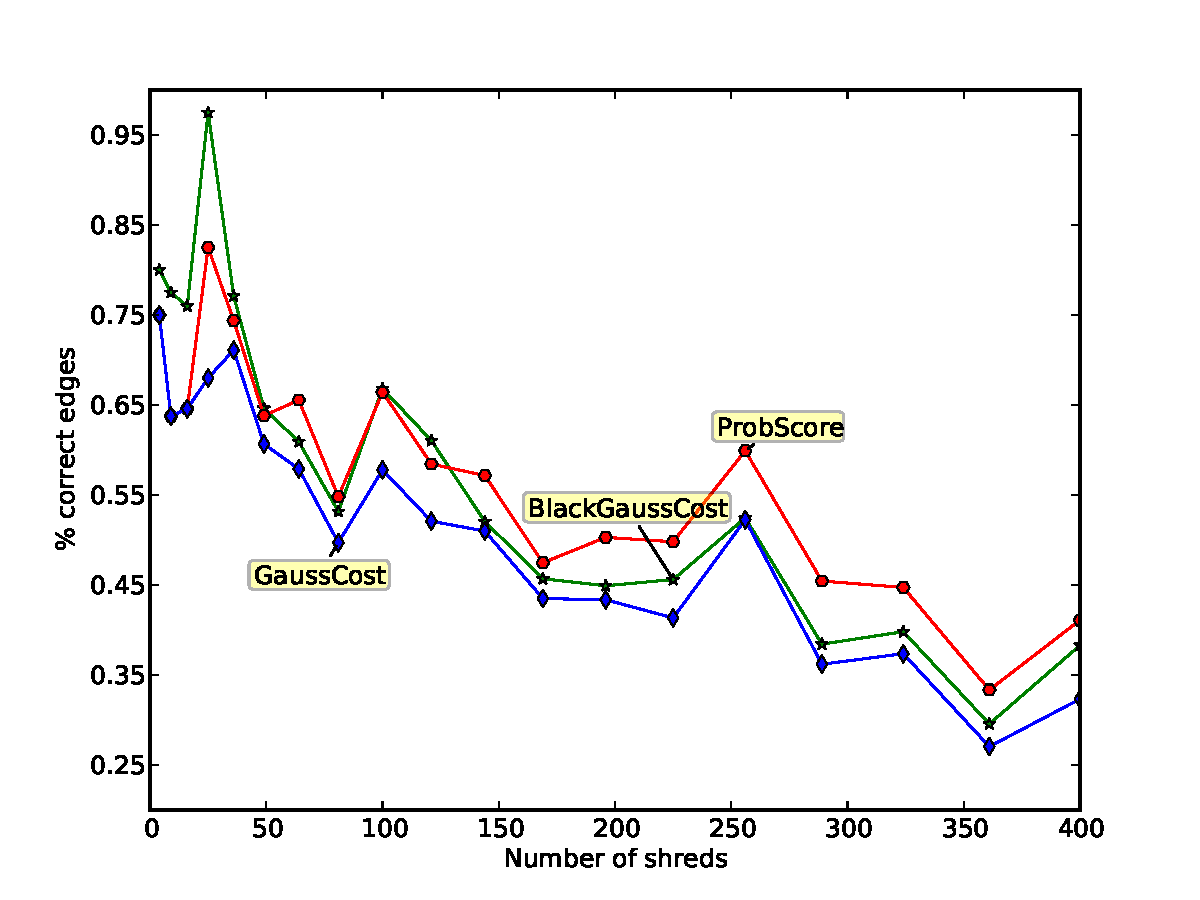
\includegraphics[width=0.8\textwidth]{costComp}
\caption{The probabilistic score has better results on medium and large instances than the cost functions presented in \cite{P1} (GaussCost) and \cite{P2} (BlackGaussCost)}
\label{fig:costComp}
\end{figure}

\subsection{Validity of predicted probabilities}
As mentioned in the Motivation, there is another(perhaps more natural) evaluation that we can perform. Namely comparing the predicted and observed probabilities for our predicted edge matches. The observed probabilities are calculated exactly as in the previous section, and the predicted probabilities are recorded for every predicted match. 

The formula $bucket = \lfloor prob * 10 + 0.5\rfloor$ is used to place the predicted probabilities into one out of a total of 10 buckets. The observed and predicted probabilities are then averaged within each bucket, and the process is repeated for different number of shreds. The resulting graph is Figure \ref{fig:probComp}.
\begin{figure}[h]
\centering
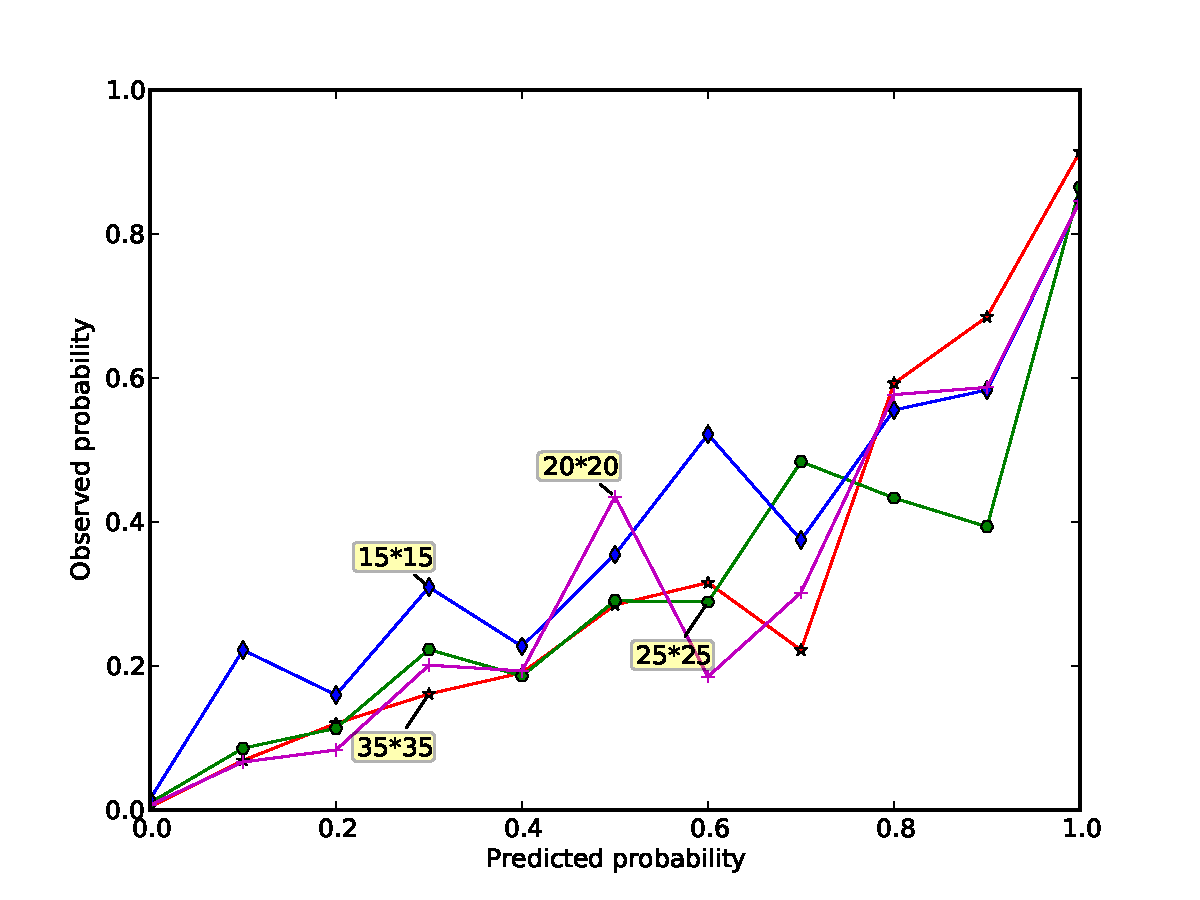
\includegraphics[width=0.8\textwidth]{predObsProb}
\caption{The labels show the number of cross-cur shreds. As the number of shreds increases the correlation between the predicted and observed probability diminishes. However the overall shape of the curve is still generally increasing, so a higher predicted probability will usually translate into a higher observed probability and for large predicted probabilities the method is quite accurate}
\label{fig:probComp}
\end{figure}

\subsection{Robustness}
Another important aspect worth evaluating is the robustness of the method. When used in real life situations it is unlikely that documents will always be high-resolution, perfectly cut into shreds and completely smudge-free. In order to test this, the results obtained on an image are compared to those obtained when various types of noise are added to the image. The types of noise analysed are: downsampling, flipping random pixels and shuffling random pixels around their original position (see Figure \ref{fig:noiseTypes}). 

\begin{figure}[h]
        \centering
        \begin{subfigure}[b]{0.4\textwidth}
                \centering
                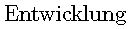
\includegraphics[width=\textwidth]{EntOrig}
                \caption{Original image}
        \end{subfigure}
        ~ 
        \begin{subfigure}[b]{0.4\textwidth}
                \centering
                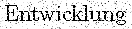
\includegraphics[width=\textwidth]{EntNoise}
                \caption{10\% of bits are randomly flipped}
        \end{subfigure}
        ~ 
        \begin{subfigure}[b]{0.4\textwidth}
                \centering
                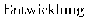
\includegraphics[width=\textwidth]{EntDown}
                \caption{The image is downsampled by a factor of 1.5}
        \end{subfigure}
        ~ 
        \begin{subfigure}[b]{0.4\textwidth}
                \centering
                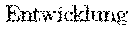
\includegraphics[width=\textwidth]{EntSpread}
                \caption{Pixels are randomly shuffled to one of their immediate neighbours}
        \end{subfigure}
        \caption{How one word of the image is modified by the various types of noise}
        \label{fig:noiseTypes}
\end{figure}

The score evaluation is run on the original and modified documents, and the results are shown in Figure \ref{fig:robustness}. As expected some performance degradation is observed in all cases. It is interesting to note that the largest reduction in performance is caused by the random pixel flipping. This can be explained by the fact that the other types of noise are restricted by the existing structure of the document, if you have a section of white pixels, neither downsampling nor shuffling can introduce a black pixel into it. The algorithm seems to suffer more from the unrestrained randomness exhibited by the flipping. The good news is that in real life scenarios most noise should not be completely random and we'd expect it to be more similar to the downsampling and shuffling types of noise than to the pixel flipping.

\begin{figure}[h]
\centering
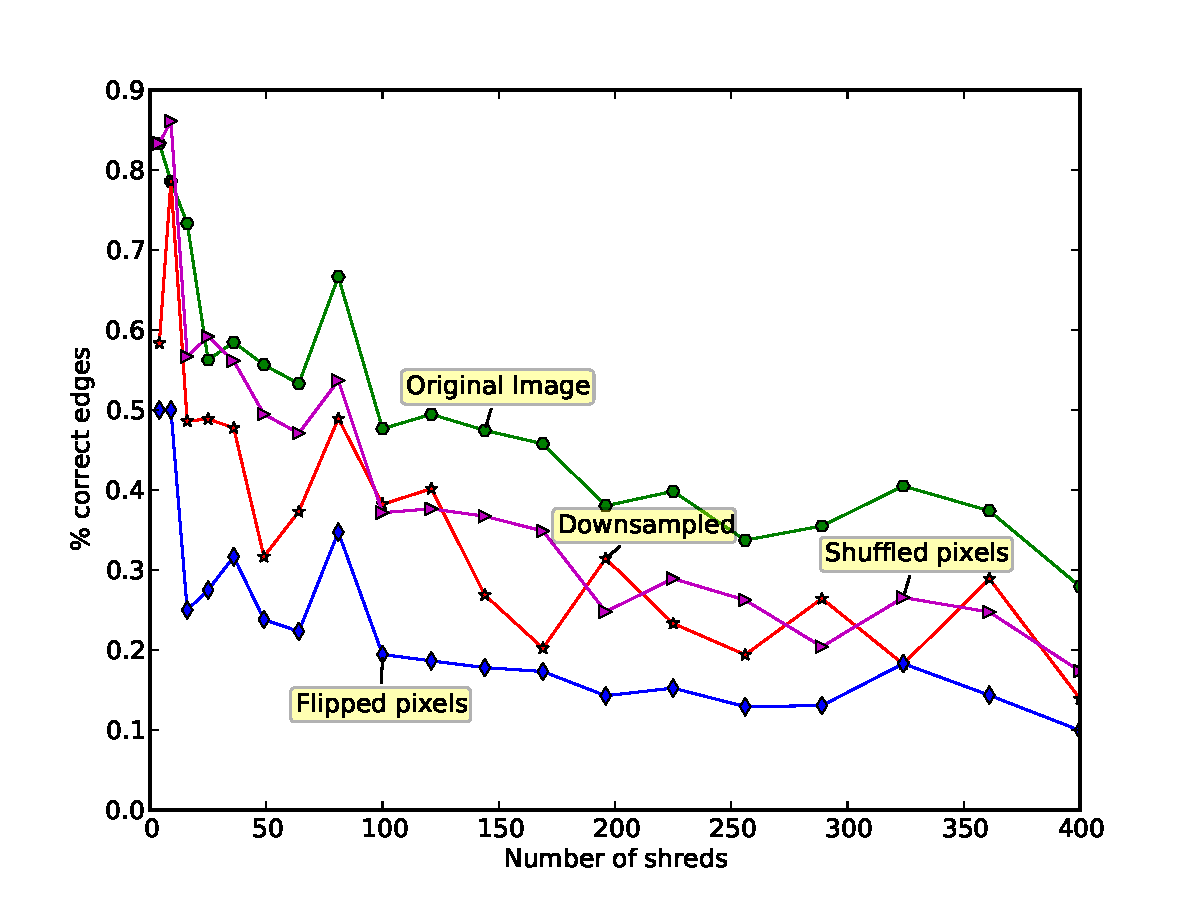
\includegraphics[width=0.8\textwidth, height=8cm]{robustness}
\caption{Degradation of performance between original image and 3 noisy images}
\label{fig:robustness}
\end{figure}

\section{Drawbacks}

Finally, we'll look at some of the flaws in the probabilistic scoring function and at some possible solutions.

\subsection{Uniformity assumption}
Learning a single set of conditional values of the form \(\Pr(p_i \mid C(p_i,E_x) \) implicitly makes the assumption that these values are relatively uniform over the whole document. This is usually a reasonable assumption to make if the documents we're interested in are all text. However this assumption is certainly not always justified. Consider the document from Figure \ref{fig:tableText}. Here we can clearly see that there are two distinct regions, the text region and the table region. An algorithm which tries to fit a single valued model to this document cannot achieve very good results, because this document cannot be described with a single set of \(\Pr(p_i \mid C(p_i,E_x) \) values. The problem will only be compounded if we're looking at multiple shredded pages from possibly different documents.

\begin{figure}[h]
\centering
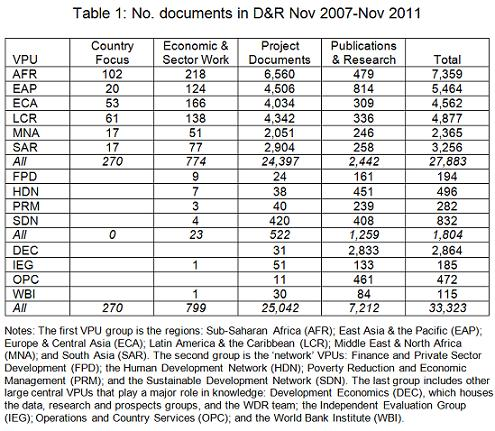
\includegraphics[width=10cm]{tableText}
\caption{A document in which the uniformity assumption is wrong.}
\label{fig:tableText}
\end{figure}

The obvious solution here is to make the probabilistic model complex enough to remove the uniformity assumption. In theory this could also help reduce the problem size, by separating the documents into smaller uniform regions. However, avoiding overfitting might be difficult in this scenario. For instance, we wouldn't want the model to decide that every boldfaced piece of text belongs together in a separate uniform region.

\subsection{Lack of symmetry}
If \(E_x\) and \(E_y\) are two edges and \(E_x^{rot}\) and \(E_y^{rot}\) are the previous edges rotated by \(180^\circ\) then we might reasonably expect that \[\forall E_x \forall E_y \Pr(E_x,E_y) = \Pr(E_y^{rot},E_x^{rot})\] This would be a good property to have, since we are essentially comparing the exact same edge matching in both situations. However, the current probabilistic model offers no such guarantee. In particular the probabilistic model cannot guarantee that \(P(E_x,E_y) = P(E_y^{rot},E_x^{rot}) \) because it is not assured (and indeed quite unlikely) that enough data was present for these two conditional probabilities to have converged to the same value.

Depending on the situation this deficiency could be ignored. It is possible, however, that the search function being employed will assume the score to be symmetric. In that case, the best solution seems to be to calculate both \(\Pr(E_x,E_y)\) and  \(\Pr(E_y^{rot},E_x^{rot})\) and re-assign both probabilities to some number in between the 2 original probabilities (arguments could be made for either $min$, $max$ or $avg$). Care should be taken that this re-assignment is done before the normalization step, otherwise the values will no longer add up to 1.

\subsection{Ignoring non-edge information}
This problem is common to both the probabilistic score and all the cost functions presented above. It is also the hardest to fix. Figure \ref{fig:fakeMatch} shows an error made on a 5x5 cross-cut document. It is interesting to notice how even in a document cut into only 25 pieces such a convincing false match can occur. As the size of the shreds and therefore the amount of information available to our scoring function decreases further we can expect a huge number of such mistakes, making reconstruction of any non-trivial cross-cut document problematic.

\begin{figure}[h]
\centering
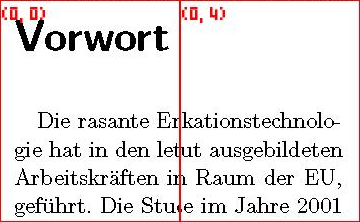
\includegraphics[width=0.6\textwidth]{conf}
\caption{An incorrect match that would be very difficult to detect by a cost/score function which only looks at the edge pixels}
\label{fig:fakeMatch}
\end{figure}

The solution here likely involves combining multiple scoring functions looking at different sets of features, both higher and lower level. Luckily, as mentioned above, the probabilistic score can easily accommodate any such scoring functions as long as they can express their result as a probability. A few possible higher level scoring functions are discussed *somewhere*. \todo{link to that part}

